% CREATED BY DAVID FRISK, 2016

% COVER PAGE
\begin{titlepage}
\newgeometry{top=3cm, bottom=3cm,
			left=2.25 cm, right=2.25cm}	% Temporarily change margins		
			
% Cover page background 
\AddToShipoutPicture*{\backgroundpic{-4}{56.7}{figure/auxiliary/frontpage_eng.pdf}}
\addtolength{\voffset}{2cm}

% Cover picture (replace with your own or delete)		
\begin{figure}[H]
\centering
\vspace{2cm}	% Adjust vertical spacing here
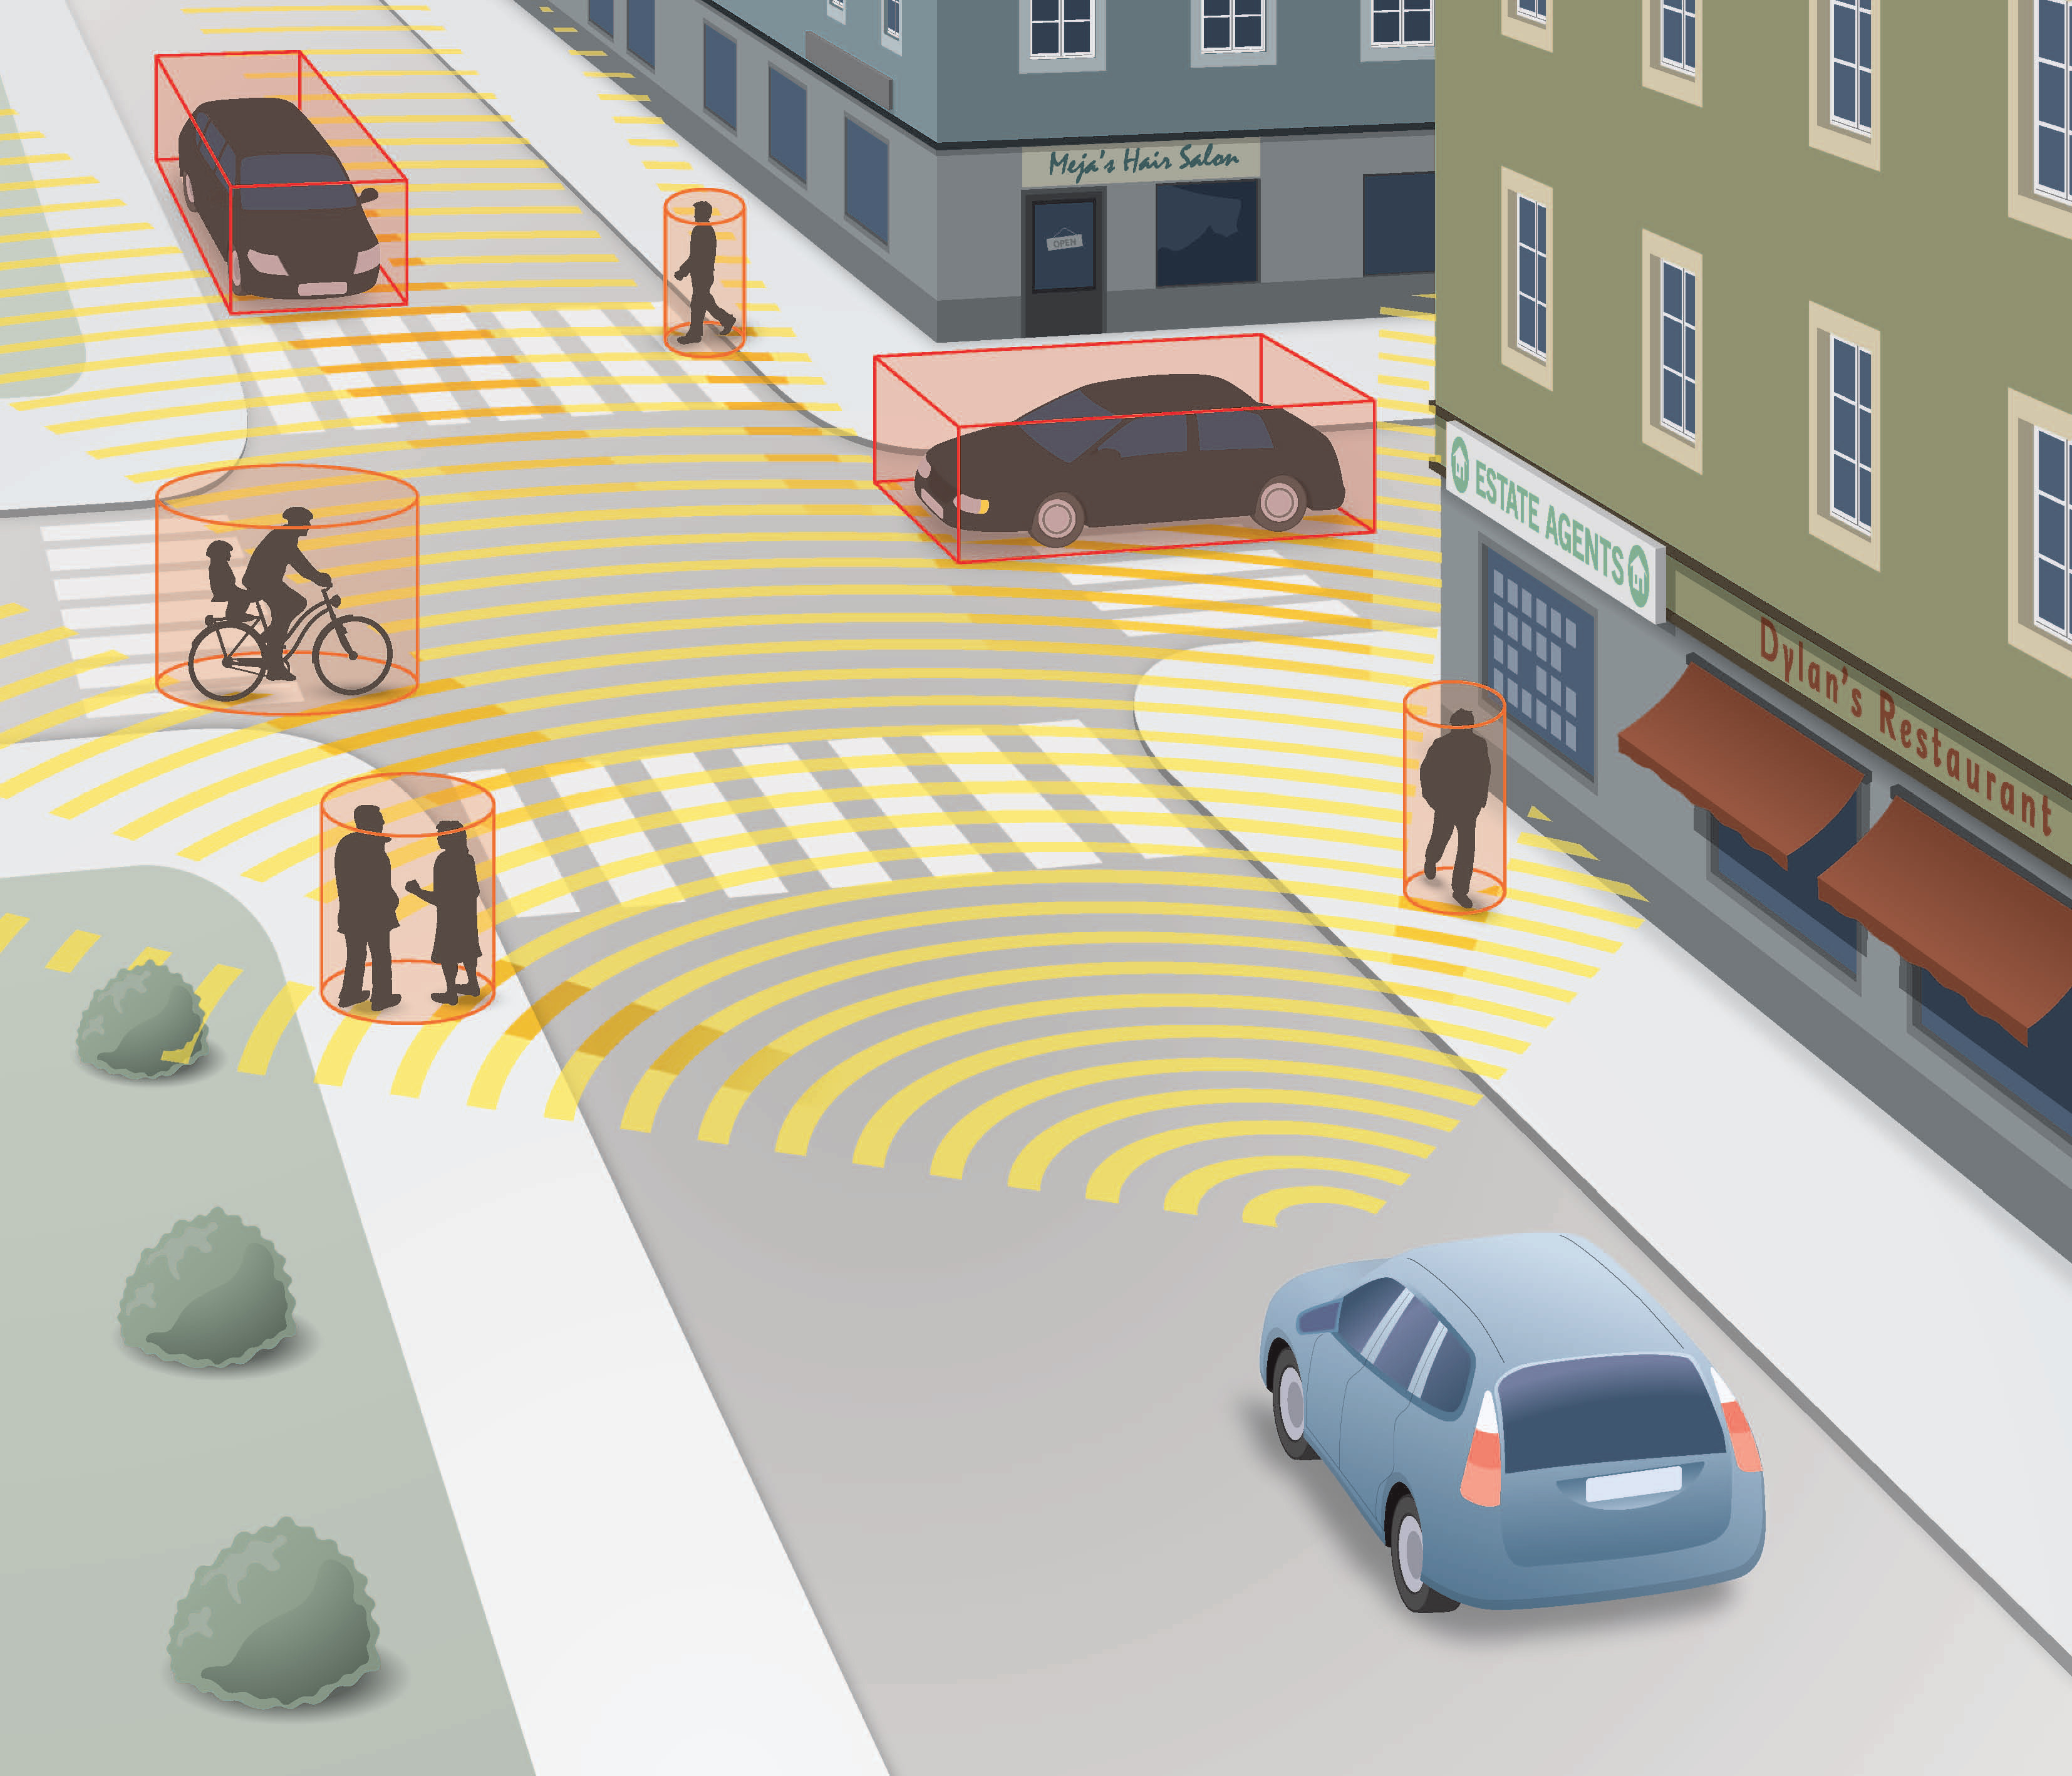
\includegraphics[width=0.7\linewidth]{figure/cover}
\end{figure}

% Cover text
\mbox{}
\vfill
\renewcommand{\familydefault}{\sfdefault} \normalfont % Set cover page font
\textbf{{\Huge 	Poisson Multi-Bernoulli Filter for	\\[0.2cm] 
				Multiple Extended Target Tracking }} 	\\[0.5cm]
{\Large }\\[0.5cm]
Master's thesis in Communication Engineering \setlength{\parskip}{1cm}

{\Large YUXUAN XIA} \setlength{\parskip}{2.9cm}

Department of Signals and Systems \\
\textsc{Chalmers University of Technology} \\
Gothenburg, Sweden 2017

\renewcommand{\familydefault}{\rmdefault} \normalfont % Reset standard font
\end{titlepage}


% BACK OF COVER PAGE (BLANK PAGE)
\newpage
\restoregeometry
\thispagestyle{empty}
\mbox{}


% TITLE PAGE
\newpage
\thispagestyle{empty}
\begin{center}
	\textsc{\large Master's thesis 2017:NN}\\[4cm]		% Report number given by department 
	\textbf{\Large Poisson Multi-Bernoulli Filter for Multiple Extended Target Tracking} \\[1cm]
% 	{\large A Subtitle that can be Very Much Longer if Necessary}\\[1cm]
	{\large YUXUAN XIA}
	
	\vfill	
	% Logotype on titlepage	
	\begin{figure}[H]
	\centering
	% Remove the following line to remove the titlepage logotype
	
\includegraphics[width=0.2\pdfpagewidth]{figure/auxiliary/logo_eng.pdf} \\	
	\end{figure}	\vspace{5mm}	
	
	Department of Signals and Systems \\
	\emph{Division of Communication Systems}\\
% 	Name of research group (if applicable)\\
	\textsc{Chalmers University of Technology} \\
	Gothenburg, Sweden 2017 \\
\end{center}


% IMPRINT PAGE (BACK OF TITLE PAGE)
\newpage
\thispagestyle{plain}
\vspace*{4.5cm}
Poisson Multi-Bernoulli Filter for Multiple Extended Target Tracking\\
% A Subtitle that can be Very Much Longer if Necessary\\
YUXUAN XIA \setlength{\parskip}{1cm}

\copyright ~ YUXUAN XIA, 2017. \setlength{\parskip}{1cm}

Supervisor: Karl Granst{\"o}m, Lennart Svensson, Department of Signals and Systems\\
Examiner: Lennart Svensson, Department of Signals and Systems \setlength{\parskip}{1cm}

Master's Thesis 2017:NN\\	% Report number given by department 
Poisson Multi-Bernoulli Filter for Multiple Extended Target Tracking\\
% Name of research group (if applicable)\\
Chalmers University of Technology\\
SE-412 96 Gothenburg\\
Telephone +46 31 772 1000 \setlength{\parskip}{0.5cm}

\vfill
% Caption for cover page figure if used, possibly with reference to further information in the report
Cover: Urban scene with multiple moving objects. The blue vehicle must be able to keep track of all the moving objects, e.g., pedestrians, cars, bicycles, in order to operate safely. Figure source from \cite{rfsextended}. \setlength{\parskip}{0.5cm}

Typeset in \LaTeX \\
Printed by [Chalmers University of Technology]\\
Gothenburg, Sweden 2017

